\chapterauthor{thomas mcandrew}{Lehigh University}
%\chapterauthor{Second Author}{Second Author Affiliation}
\chapter{Single covariate linear regression and conditional expected value and variance}
\hspace{1mm}

\section{Introduction}\label{intro}

Regression is likely one of the most important concepts in modern statistical data analysis. 
Thousands if not tens of thousands scientific analyses depend on regression to understand the relationship between one or more variables and an outcome of interest and to make predictions about future outcomes given a new, not yet seen observation in nature.
The regression approach to model building begins with a univariate distribution---often a familiar distribution---and then allows the parameters of that distribution to depend on observed data.

\section{A new data, sampling setup}\label{intro}

Previous to this chapter our typical statistical setup assumed that our data was a set of the form $\mathcal{D} = \{ x_{1},x_{2},x_{3}, \cdots, x_{n} \}$ where we collected a single piece of information from each observation. 
Our statistical model then assumed that these observations were generated from corresponding random variables $X_{1}, X_{2}, \cdots, X_{n}$ that were independent and identically distributed.

Our new setup will consider collecting one additional piece of information from each observation
\begin{equation}
    \mathcal{D} = \{ (x_{1},y_{1}), (x_{2},y_{2}), (x_{3},y_{3}), \cdots (x_{n},y_{n})  \}
\end{equation}
Our statistical setup will assume that the $y$ data in the second position of each tuple above is the outcome of interest and that this data was sampled from a set of corresponding random variables. 
We will not consider the $x$ data as being generated from corresponding random variables. 
The $x$ data is thought of as fixed.
Our statistical setup is 
\begin{equation}
    (x_{1}, Y_{1}),(x_{2}, Y_{2}),(x_{3}, Y_{3}), \cdots, (x_{n}, Y_{n}) 
\end{equation}
where we assume that $Y_{i}$ are independent and identically distributed.
We will assign to the random variables $Y$ a probabilistic distribution.

\ex We are asked to collect data on patients who are admitted to the hospital to test the hypothesis that those who are hospitalized with influenza are more likely to be under the age of 3 or over the age of 65. 
A single observation will then contain two pieces of information: (i) whether the patient admitted to the hospital has confirmed influenza and (ii) whether the patient is younger than 3 or older than 65 or in between these ages. 
Our dataset will look like $\mathcal{D} = \{(r_{1},i_{1}),(r_{2},i_{2}),(r_{3},i_{3}),\cdots,(r_{n},i_{n})  \}$ where the variable $r$ is the value one when a patient is younger than 3 or older than 65 and the value zero otherwise, and the variable $i$ is the value one when the patient was infected with influenza and the value zero otherwise.

\section{Conditional distributions}\label{intro}

We must make concise what we mean when we suppose that values of $x$ impact our outcome of interest $Y$.
Let us define the distribution of the random $Y$, conditional on the observation $x$, or $Y | x$, as a probability mass function or density function that produces different probabilities over the support of $Y$ for different values of the observation $x$.

\ex Assume that $Y$ has a geometric distribution with the following modification
\begin{align}
    P(Y=y | x) = g(x) ( 1-g(x) )^{y-1}  
\end{align}
where the function $g(x)$ must be between the values 0 and 1 (Why?). 
We could write the above as $Y | x \sim \text{Geom}( g(x) )$ and say that the distribution of $Y$ is conditional on the value of $x$.
When $g(x) = 0.2$ then $P(Y=5) = 0.08$ and when $g(x) = 0.9$ then $P(Y=5) = 0.00009$.

\section{Conditional expectation and variance}\label{intro}

For a discrete random variable, the conditional expectation of a random variable $Y|x$ is defined as 
\begin{align}
    \mathbb{E}(Y|x) = \sum_{ y \in supp(Y) } y p(y |x) 
\end{align}
and for a continuous random variable is defined as 
\begin{align}
    \mathbb{E}(Y|x) = \int_{y \in supp(Y)} y f(y | x)  \; dy
\end{align}
where $f$ is the conditional probability density corresponding to $Y|x$.

Because the distribution of $Y$ depends on $x$ then the expected value too will depend on the observed $x$ value.
However, we assume that the observation $x$ is not random, the $x$ value is a fixed observation. This assumption makes computing the conditional expectation easier.

\ex Suppose that $supp(Y) = \{-1,0,1\}$ and that $x$ can take the values 0 or 1. Further assume the conditional probability distribution
\begin{table}[ht!]
    \centering
    \begin{tabular}{c|cc}
             &   x=0 & x=1  \\
        \hline
        y=-1 &  0.10 & 0.40\\ 
        y=0  &  0.50 & 0.30\\
        y=1  &  0.40 & 0.30
    \end{tabular}
    \caption{Conditional distribution of $Y|x$}
\end{table}
Then 
\begin{align}
    \mathbb{E}(Y|x=0) &= \sum_{y \in \{-1,0,1\}} y p(y|x=0) \\ 
                      &= (-1) 0.1 + (0) 0.50 + (1) 0.40 \\ 
                      &= -0.1 + 0.40 = 0.30 
\end{align}
and 
\begin{align}
    \mathbb{E}(Y|x=1) &= \sum_{y \in \{-1,0,1\}} y p(y|x=1) \\ 
                      &= (-1) 0.4 + (0) 0.30 + (1) 0.30 \\ 
                      &= -0.4 + 0.30 = -0.10 
\end{align}

For a discrete random variable, the conditional variance of a random variable $Y|x$ is defined as 
\begin{align}
    \mathbb{V}(Y|x) = \sum_{ y \in supp(Y) } \left[y - \mathbb{E}(Y | x)\right]^{2} p(y |x) 
\end{align}
and for a continuous random variable is defined as 
\begin{align}
    \mathbb{V}(Y|x) = \int_{y \in supp(Y)} \left[y - \mathbb{E}(Y | x)\right]^{2} f(y | x)  \; dy
\end{align}
where $f$ is the conditional probability density corresponding to $Y|x$.

\ex Lets continue with the above example and compute $V(Y|x)$. 
\begin{align}
    \mathbb{V}(Y|x=0) &= \sum_{y \in \{-1,0,1\}} [ y - \mathbb{E}(Y|x=0)  ]^{2} p(y|x=0) \\ 
                      &= (-1 - 0.30)^{2} 0.1 + (0 - 0.30)^{2} 0.50 + (1-0.30)^{2} 0.40 \\ 
                      &= 0.41
\end{align}


\section{Parameters as a function of observations}\label{intro}

\textbf{Single covariate linear regression} assumes that given a sample $(Y_{1}, x_{1}), (Y_{2}, x_{2}), (Y_{3}, x_{3}), \cdots, (Y_{n}, x_{n}) $ that the conditional distribution of $Y$ given $x$ follows a normal distribution
\begin{align}
    Y | x \sim \mathcal{N}\left( \mu(x), \sigma^{2} \right)
\end{align}
where $\mu(x) = \beta_{0} + \beta_{1} x$, and $\beta_{0}$ and $\beta_{1}$ are parameters that take values in $\mathcal{R}$.
The above is sometimes called \textbf{the probability form} of linear regression.
In probability form we emphasize that our target of interest is modeled as a random variable $Y$ and make explicit that this random variable is expected to be distributed normal.

Because $\beta_{0}$ and $\beta_{1}$ are constant, and because $x$ is a fixed, constant observation then $\mu(x) = \beta_{0} + \beta_{1}x$ is a constant.
Remember that it is easy to translate normal distributions by a constant.
Lets choose to add and subtract the constant $(\mu(x))$

The \textbf{conditional expectation for single covariate regression} can be computed by recognizing that $\mu(x)$ is a constant, 
\begin{align}
    \mathbb{E}(Y|x) = \mu(x) = \beta_{0} + \beta_{1}x,
\end{align}
and the \textbf{conditional variance for single covariate regression} can also be computed as 
\begin{align}
    \mathbb{V}(Y|x) = \sigma^{2}
\end{align}
We see that the variance does not depend on $x$ and remains constant.


\begin{align}
    Y |x \sim \mathcal{N}(\mu(x), \sigma^{2}) \\ 
    Y |x  = Y |x + \mu(x) - \mu(x)
\end{align}
Lets define a new random variable $\epsilon =  Y |x - \mu(x)$. 
Then 
\begin{align}
    Y |x  = \mu(x) + \epsilon\\
\end{align}
We can look closer at the distribution for $\epsilon$
The random variable $\epsilon$ is a translation of $Y|x$. 
\begin{align}
    \epsilon \sim \mathcal{N}(\mu(x), \sigma^{2}) - \mu(x)\\
    \epsilon \sim \mathcal{N}(\mu(x)-\mu(x), \sigma^{2}) \\
    \epsilon \sim \mathcal{N}(0, \sigma^{2}) 
\end{align}
Finally we see that we can rewrite our linear regression as 
\begin{align}
    Y |x  = \mu(x) + \epsilon\\
    \epsilon \sim \mathcal{N}(0, \sigma^{2})
\end{align}
This form for linear regression---the conditional expected value plus an error term~($\epsilon$)---is often called the \textbf{model form} for linear regression.
Model form emphasizes, $\mu(x)$, often thought of as how you think $x$ and $Y$ are associated with one another.

Linear regression supposes that there exists a linear relationship between the random variable $Y$ and the observations $x$. 
One way to investigate whether or not a linear relationship between $Y$ and $x$ appears reasonable is to draw a scatter plot. 

Given a dataset $\mathcal{D} = \{ (x_{1}, y_{1}),(x_{2}, y_{2}), \cdots (x_{n}, y_{n}) \}$
A scatter plot first draws a x and y axis on the cartesian coordinate plane. 
The second step iterates through each data point $(x_{i},y_{i})$ and places a dot on the plane at $(x_{i},y_{i})$. If it appears that a straight line may well explain the association between $x$ and $\mathbb{E}(Y|x)$ then a linear regression model could be fit to this data. 

\section{The residual, diagnostics, and LINE assumptions}

Single covariate linear regression is a model to help us understand the relationship between two covariates that we call, $y$ and $x$. 
Rarely, if ever, will our model perfectly describe our observed data. 
In this case, we will need to evaluate how well our model fits our observed data and if single covariate regression is a reasonable, or un-reasonable, model.
Evaluating how well our statistical model describes an observed dataset is called \textbf{diagnostics}.

Assume that we can find optimal estimates for our parameters $\beta_{0}, \beta_{1},$ and $\sigma^{2}$. 

\subsection{Residuals, fitted values, and Normality}

The random variable $\epsilon$ that we defined for the model form of single covariate linear regression is exact, assuming that we know all of our parameter values.
However, in most cases we will not be given the exact parameter values. 
Instead we are handed a dataset and asked to estimate our parameters.
In this case, we will never know the true distribution of our error term $\epsilon_{i}$ that corresponds to a specific $x_{i}$ value. 
We can estimate the error term $\epsilon$ at the value $x$ given: (i) estimates for our parameters and (ii) a datapoint $(x, y)$ from our dataset. 
Given a datapoint $d = (x,y)$, a \textbf{residual} is the difference between the truly observed $y$ and an estimate of $y$, $\hat{y}$, or $\hat{\epsilon} = y - \hat{y}$.

Given estimates for our parameters $(\beta_{0}, \beta_{1}, \sigma^{2})$, a \textbf{fitted value} to a datapoint $d = (x,y)$ is $\hat{y} = \hat{\beta_{0}} + \hat{\beta_{1}} x $.

Residuals and fitted values can be used to test the assumptions of our regression model. 
If our regression captures the variability in our dataset well then the residuals $\hat{\epsilon}_{i}$ should behave similarly to the true error terms $\epsilon_{i} \sim \mathcal{N}(0,\sigma^{2})$. 

\subsubsection{Linearity}

One assumption about single covariate linear regression to evaluate is that the relationship between $x$ and the conditional expected value of $Y$, $\mathbb{E}(Y|x)$ is linear.
Single covariate regression assumes that $\mathbb{E}(Y|x) = \beta_{0} + \beta_{1} x$ and that $\mathbb{E}(\epsilon) = 0$ for any choice of $x$.

To test for linearity we can plot for each $x$ value the corresponding residual $\hat{\epsilon} = y - (\beta_{0} + \beta_{1} x)$.
If single covariate regression sufficiently explains the relationship between our random variables $Y$ and fixed data $x$ then we could expect that this plot has residuals values centered around zero for all choice of $x$.
If single covariate regression does not fit the data well then our residuals will not be centered around zero.

\ex Suppose we collect the following dataset 
\begin{table}[ht!]
    \centering
    \begin{tabular}{c|c}
        x & y    \\
        \hline
     0.44 & 1.23 \\
     0.50 & 1.19 \\
     0.83 & 1.26 \\ 
     0.41 & 1.26 \\
     0.03 & 0.87 \\
     0.20 & 0.87 \\
     0.98 & 1.45 \\
     0.37 & 1.28 \\
     0.80 & 1.31 \\
     0.99 & 1.69 \\
    \end{tabular}
    \caption{Data simulated from the model $y \sim \mathcal{N}(1+0.5x, 0.15)$\label{tab.diag}}
\end{table}
and we compute estimates for our parameters $\hat{\beta_{0}} = 0.88$, $\hat{\beta_{1}} = 0.64$, and $\hat{\sigma^{2}} = 0.12$.

We can compute 10 fitted values and 10 residuals corresponding to our 10 collected data points
\begin{table}[ht!]
    \centering
    \begin{tabular}{c|c|c|c}
        x & y & $\hat{y}$ & $\hat{\epsilon}$    \\
        \hline
     0.44 & 1.23 & 1.16 & 0.07 \\
     0.50 & 1.19 & 1.20 & -0.01\\
     0.83 & 1.26 & 1.41 & -0.15\\ 
     0.41 & 1.26 & 1.14 & 0.12 \\
     0.03 & 0.87 & 0.90 & -0.03\\
     0.20 & 0.87 & 1.01 & -0.14\\
     0.98 & 1.45 & 1.51 & -0.06\\
     0.37 & 1.28 & 1.12 & 0.16\\
     0.80 & 1.31 & 1.39 & -0.08\\
     0.99 & 1.69 & 1.51 & 0.18\\
    \end{tabular}
    \caption{Data simulated from the model $y \sim \mathcal{N}(1+0.5x, 0.15)$\label{tab.diag}}
\end{table}

By plotting our fitted values $\hat{y}$, which depend on $x$, against our residuals we can visualize whether or not our residuals $\hat{\epsilon}$ are centered around zero. 
If the residuals show a pattern that does not appear to be centered around zero than the relationship between $x$ and $Y$ may not be linear.

\begin{figure}
    \centering
    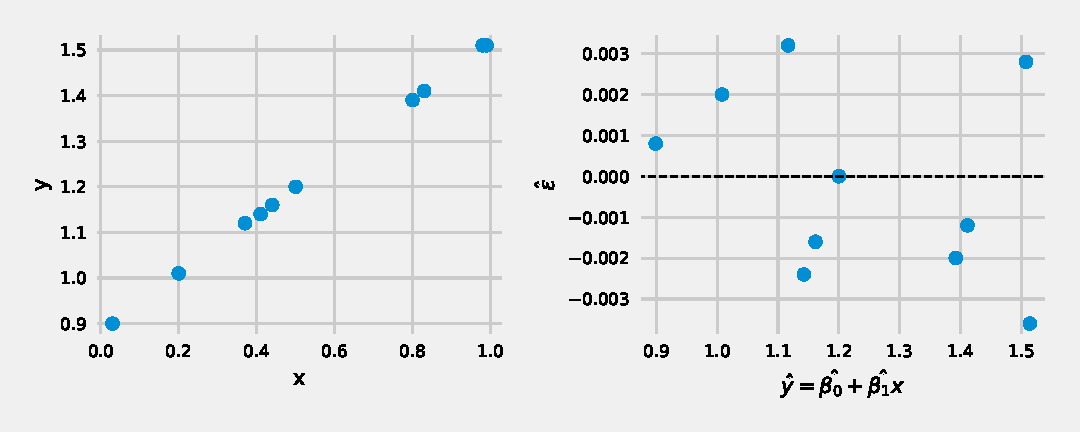
\includegraphics[width=\textwidth]{chapters/chapter7/ch6_residuals_vs_fitted.pdf}
    \caption{(Left) Scatter plot of $(x,y)$ pairs from the above dataset.
    (Right) Scatterplot of residuals versus fitted values. \label{fig.residualsDiag}}
\end{figure}

We see from the plot of $x$ vs $y$ that the relationship between $x$ and $y$ looks linear. In addition, the scatter plot of the fitted values versus residuals also looks like the residuals show not particular pattern and are centered around zero for all fitted values.

\subsubsection{Equal variance}

A plot of fitted values versus residuals can also be used to assess whether the assumption that the error $(\epsilon)$ is distributed $\mathcal{N}(0,\sigma^{2})$ according to a normal distribution with \textbf{the same variance for all values of $x$}.
This assumption is often called the equal variances assumption.

Below we generated 100 $(x,y)$ pairs of observed data points. 
We estimated our parameter values~(more on this later) and then computed fitted values and residuals. 
Again we plotted a scatterplot of $x$ vs $y$ and a plot of fitted values vs residuals.
We see from the residuals vs fitted values that it appears that the residuals move further away from zero as $x$ values increase.
This indicates that the \textbf{equal variances} assumption may not best describe our data.

\begin{figure}
    \centering
    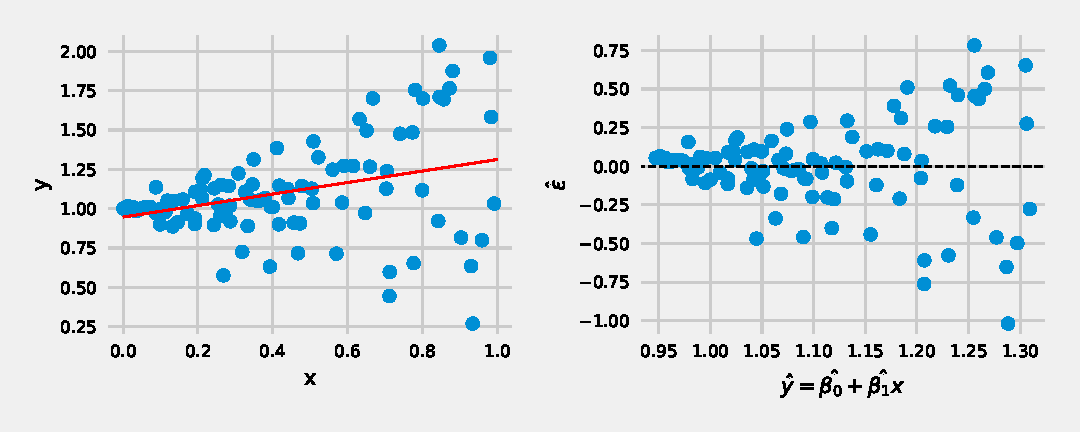
\includegraphics[width=\textwidth]{chapters/chapter7/ch6_residuals_vs_fitted__extravar.pdf}
    \caption{(Left) Scatter plot of 100 $(x,y)$ pairs from the above dataset with the line (red) $\hat{\mathbb{E}(Y|x)} = \hat{\beta_{0}} + \hat{\beta_{1}}x$.
    (Right) Scatterplot of residuals versus fitted values. \label{fig.residualsDiag}}
\end{figure}

\subsection{Independence}

The independence between data points $d_{i} = (x_{i}, y_{i})$ and $d_{j} = (x_{j}, y_{j})$ for any $(i,j)$ can be tested with a sequence vs residual plot. 
For this plot we graph residuals versus a variable that indicates when in time the data was collected. 
For example, we may decide to plot the time the data point was collected vs residual, or we can rank the data by the time it was collected and plot the rank vs residual.
For single covariate linear regression, we expect that there does not exist a relationship between when the data was collected and the residuals.
We assume that errors $\epsilon$ are independent from one another.
If there is a relationship between when the data was collected and residuals then this may indicate the data points are not independent.

\begin{figure}
    \centering
    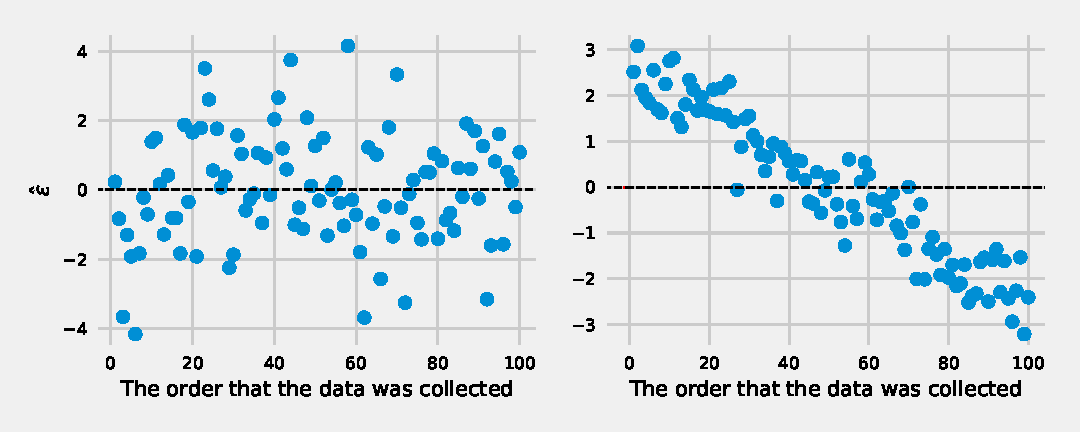
\includegraphics[width=\textwidth]{chapters/chapter7/ch6_residuals_vs_sequence.pdf}
    \caption{(Left) Scatter plot of 100 $(\text{order},\hat{\epsilon})$ pairs from a dataset where data was generated independently. 
    (Right) Scatterplot of the order that the data was collected versus residuals for data that was generated dependently. \label{fig.residualsDiag}}
\end{figure}


\section{Sums of squares}

Up until this point we assumed that we can compute estimates for $\beta_{0}$ and for $\beta_{1}$, but we have not yet discussed methods to compute estimates for these parameters. 
The first method we will explore is called \textbf{minimizing the sums of squares} or is often also called \textbf{least squares}.

Given a dataset $\mathcal{D} = \{ (x_{1},y_{1}), (x_{2},y_{2}), \cdots (x_{n},y_{n}) \}$ and a single covariate regression model $Y_{i} = \mu(x) + \epsilon$ where $\epsilon \sim \mathcal{N}(0,\sigma^{2})$, the least squares estimates for $\beta_{0}$ and $\beta_{1}$ are the values that minimize 
\begin{align}
    SS(\beta_{0}, \beta_{1}) = \sum_{i=1}^{N} \left[ y_{i} - \left(\beta_{0} + \beta_{1}x_{i} \right)  \right]^{2}
\end{align}
The function $SS(\beta_{0}, \beta_{1})$ is called the "sums of squares" function.
To minimize $SS(\beta_{0}, \beta_{1})$ we will
\begin{enumerate}
    \item Treat $\beta_{1}$ as a constant, treat $\beta_{0}$ as a variable, take the derivative and set that equation to zero. 
    \item Treat $\beta_{0}$ as a constant, treat $\beta_{1}$ as a variable, take the derivative and set that equation to zero. 
    \item Solve the above two equations for $\beta_{0}$ and $\beta_{1}$.
\end{enumerate}

\subsection{ $\beta_{0}$ as the variable and $\beta_{1}$ as a constant}

Because the SS function is a sum of similar terms, we can compute the derivative for one term and then add each term together. 

\begin{align}
    SS(\beta_{0})' &= \left\{ \sum_{i=1}^{N} \left[ y_{i} - \left(\beta_{0} + \beta_{1}x_{i} \right)  \right]^{2} \right \}' \\
    &=  \sum_{i=1}^{N} \left\{ \left[ y_{i} - \left(\beta_{0} + \beta_{1}x_{i} \right)   \right]^{2}\right \}
\end{align}

The goal then is to compute the derivative of 
\begin{align}
    SS(\beta_{0}) = \left[ y_{i} - \left(\beta_{0} + \beta_{1}x_{i} \right)  \right]^{2}
\end{align}
We will need to use the chain rule
\begin{align}
    SS(\beta_{0}) &= \left[ h(\beta_{0}) \right]^{2} \\ 
    h(\beta_{0}) &= y_{i} - \left(\beta_{0} + \beta_{1}x_{i} \right) \\
\end{align}

The derivative of 
\begin{align}
    SS(\beta_{0}) &= \left[ h(\beta_{0}) \right]^{2} \\
\end{align}
is 
\begin{align}
    SS(\beta_{0}) &= 2\left[ h(\beta_{0}) \right] \\
\end{align} and the derivative of 
\begin{align}
    h(\beta_{0}) &= y_{i} - \left(\beta_{0} + \beta_{1}x_{i} \right) \\
\end{align}
is 
\begin{align}
    h(\beta_{0})' &= - 1,
\end{align}
and so the derivative of $SS(\beta_{0})$ is 
\begin{align}
    SS(\beta_{0})' &= \sum_{i=1}^{N} 2\left[ h(\beta_{0}) \right] \times (-1) \\ 
                   &= \sum_{i=1}^{N} -2\left[y_{i} - \left(\beta_{0} + \beta_{1}x_{i} \right) \right]
\end{align}

We can set this equation equal to zero and solve for $\beta_{0}$ to find the least squares estimate for $\beta_{0}$
\begin{align}
    \sum_{i=1}^{N} -2\left[y_{i} - \left(\beta_{0} + \beta_{1}x_{i} \right) \right] &=0 \\ 
    \sum_{i=1}^{N} \left[y_{i} - \left(\beta_{0} + \beta_{1}x_{i} \right) \right] &=0 \\
    \sum_{i=1}^{N} y_{i} - \sum_{i=1}^{N} \beta_{0} -\sum_{i=1}^{N} \beta_{1}x_{i}  &=0 \\
    \sum_{i=1}^{N} y_{i} - N \beta_{0} -\sum_{i=1}^{N} \beta_{1}x_{i}  &=0 \\
    \sum_{i=1}^{N} y_{i}  -\sum_{i=1}^{N} \beta_{1}x_{i}  &= N \beta_{0} \\
    \sum_{i=1}^{N} y_{i}  - \beta_{1}\sum_{i=1}^{N} x_{i}  &= N \beta_{0} \\
    \frac{\sum_{i=1}^{N} y_{i}}{N}  - \beta_{1}\frac{\sum_{i=1}^{N}x_{i}}{N}  &=  \beta_{0}\\
    \bar{y} - \beta_{1}\bar{x}  &=  \beta_{0}
\end{align}

The \textbf{least squares estimate for $\beta_{0}$} is 
\begin{align}
    \hat{\beta_{0}}_{\text{SS}} = \bar{y} - \beta_{1} \bar{x}
\end{align}

\subsection{ $\beta_{1}$ as the variable and $\beta_{0}$ as a constant}

Lets take the same approach for computing an estimate for $\beta_{1}$.

\begin{align}
    SS(\beta_{1})' &= \left\{ \sum_{i=1}^{N} \left[ y_{i} - \left(\beta_{0} + \beta_{1}x_{i} \right)  \right]^{2} \right \}' \\
    &=  \sum_{i=1}^{N} \left\{ \left[ y_{i} - \left(\beta_{0} + \beta_{1}x_{i} \right)   \right]^{2}\right \}
\end{align}

The goal then is to compute the derivative of 
\begin{align}
    SS(\beta_{1}) = \left[ y_{i} - \left(\beta_{0} + \beta_{1}x_{i} \right)  \right]^{2}
\end{align}
We will need to use the chain rule
\begin{align}
    SS(\beta_{1}) &= \left[ h(\beta_{1}) \right]^{2} \\ 
    h(\beta_{1}) &= y_{i} - \left(\beta_{0} + \beta_{1}x_{i} \right)
\end{align}

The derivative of 
\begin{align}
    SS(\beta_{1}) &= \left[ h(\beta_{1}) \right]^{2}
\end{align}
is 
\begin{align}
    SS(\beta_{1}) &= 2\left[ h(\beta_{1}) \right] 
\end{align} and the derivative of 
\begin{align}
    h(\beta_{1}) &= y_{i} - \left(\beta_{0} + \beta_{1}x_{i} \right) 
\end{align}
is 
\begin{align}
    h(\beta_{0})' &= -x_{i},
\end{align}
and so the derivative of $SS(\beta_{1})$ is 
\begin{align}
    SS(\beta_{1})' &= \sum_{i=1}^{N} 2\left[ h(\beta_{1}) \right] \times (-x_{i}) \\ 
                   &= \sum_{i=1}^{N} -2x_{i}\left[y_{i} - \left(\beta_{0} + \beta_{1}x_{i} \right) \right]
\end{align}

We can set this equation equal to zero and solve for $\beta_{1}$ to find the least squares estimate for $\beta_{1}$
\begin{align}
    \sum_{i=1}^{N} -2x_{i}\left[y_{i} - \left(\beta_{0} + \beta_{1}x_{i} \right) \right] &= 0\\
    \sum_{i=1}^{N} -x_{i}\left[y_{i} - \left(\beta_{0} + \beta_{1}x_{i} \right) \right] &= 0\\
    \sum_{i=1}^{N} -x_{i} y_{i} + x_{i}\beta_{0} + \beta_{1}x^{2}_{i} &= 0\\
    \sum_{i=1}^{N} -x_{i} y_{i} + \beta_{0} \sum_{i=1}^{N} x_{i} + \beta_{1} \sum_{i=1}^{N} x^{2}_{i} &= 0\\
    \beta_{1} \sum_{i=1}^{N} x^{2}_{i} &= \sum_{i=1}^{N} x_{i} y_{i} - \beta_{0} \sum_{i=1}^{N} x_{i} \\
\end{align}

\subsection{Solving for $\beta_{0}$ and $\beta_{1}$}
At this point we have two equations and two unknowns:
\begin{align}
    \beta_{0} &= \bar{y} - \beta_{1} \bar{x} \\ 
     \beta_{1} \sum_{i=1}^{N} x^{2}_{i} &= \sum_{i=1}^{N} x_{i} y_{i} - \beta_{0} \sum_{i=1}^{N} x_{i} \\
\end{align}

We can solve the above equations and find that the least squares estimates for $\beta_{0}$ and for $\beta_{1}$ are

\begin{align}
    \hat{\beta_{1}} &= \frac{ \sum_{i=1}^{N} (x_{i} - \bar{x})(y_{i} - \bar{y})  }{ \sum_{i=1}^{N} (x_{i} - \bar{x})^{2} }\\
    \hat{\beta_{0}} &= \bar{y} - \hat{\beta_{1}} \bar{x} \\
\end{align}

\ex Suppose we collect the dataset 
\begin{table}[ht!]
    \centering
    \begin{tabular}{c|c}
        x & y \\
        \hline
        0.38 & 0.72\\
        0.04 & 1.00\\
        0.79 & 0.19\\
        0.48 & 0.69\\
        0.68 & 0.56\\
    \end{tabular}
\end{table}

We can compute the least squares estimates for $\beta_{0}$ and $\beta_{1}$ by following these steps:

\textbf{Compute $\bar{x}$ and $\bar{y}$}
\begin{align}
    \bar{x} = \frac{0.38 + 0.04 + 0.79 + 0.48 + 0.68}{5} = 0.47\\
    \bar{y} = \frac{0.72 + 1.00 + 0.19 + 0.69 + 0.56}{5} = 0.63\\
\end{align}

\clearpage
\textbf{Augment the above table with a column that computes $x_{i} - \bar{x}$ and $y_{i} - \bar{y}$}

\begin{table}[ht!]
    \centering
    \begin{tabular}{c|c|c|c }
        x & y & $(x_{i} - \bar{x})$ & $(y_{i} - \bar{y})$ \\
        \hline
        0.38 & 0.72 & -0.09 &  0.09\\
        0.04 & 1.00 & -0.43 &  0.37\\
        0.79 & 0.19 & 0.31  &  -0.44\\
        0.48 & 0.69 & 0.01  &  0.05 \\
        0.68 & 0.56 & 0.21. &  -0.07 \\
    \end{tabular}
\end{table}


\textbf{Add a column that computes  $(x_{i} - \bar{x})(y_{i} - \bar{y})$ and that computes $(x_{i} - \bar{x})^{2}$}

\begin{table}[ht!]
    \centering
    \begin{tabular}{c|c|c|c|c|c }
        x & y & $(x_{i} - \bar{x})$ & $(y_{i} - \bar{y})$ & $(x_{i} - \bar{x})(y_{i} - \bar{y})$ & $(x_{i} - \bar{x})^{2}$ \\
        \hline
        0.38 & 0.72 & -0.09 &  0.09  & -0.01 & 0.01 \\
        0.04 & 1.00 & -0.43 &  0.37  & -0.16 & 0.18 \\
        0.79 & 0.19 & 0.31  &  -0.44 & -0.14 & 0.10 \\
        0.48 & 0.69 & 0.01  &  0.05  & 0.00  & 0.0 \\
        0.68 & 0.56 & 0.21. &  -0.07 & -0.02 & 0.04 \\
    \end{tabular}
\end{table}

\textbf{Compute the sums of the last two columns and divide the second to last column by the last column to estimate $\beta_{1}$ }

\begin{align}
    \sum_{i=1}^{N} (x_{i} - \bar{x})(y_{i} - \bar{y}) &= -0.01 -0.16 - 0.14 + 0.00 - 0.02  = - 0.33 \\ 
    \sum_{i=1}^{N} (x_{i} - \bar{x})^{2} &= 0.01 + 0.18 + 0.10 + 0.0 + 0.04 = 0.33 \\ 
    \hat{\beta_{1}} &= -0.33 / 0.33 = -1
\end{align}

\textbf{Use your estimate for $\beta_{1}$ to estimate $\beta_{0}$}
\begin{align}
    \hat{\beta_{0}} &= \bar{y} - \hat{\beta_{1}} \bar{x} \\ 
    \hat{\beta_{0}} &= 0.63 - (-1)(0.47)  = 1.1
\end{align}



\section{Maximum likelihood estimates for $\beta_{0}$, $\beta_{1}$, and $\sigma^{2}$}

We must estimate three parameters for single covariate linear regression: $\beta_{0}, \beta_{1}, \sigma^{2}$.
We will take a maximum likelihood approach to estimate these three covariates in two steps.
Step one: compute the log-liklihod for a typical univariate normal distribution. Step two: convert this loglikelihood to single covariate linear regression.

Give a sample $\mathcal{D} = \{ (x_{1},y_{1}), (x_{2},y_{2}), (x_{3},y_{3}), \cdots, (x_{n},y_{n})\}$ assume that we model $Y$ as $Y_{i} \sim \mathcal{N}\left(\mu, \sigma^{2} \right)$ where $\mu$ does not depend on $x$ observations. 

Then the likelihood can be computed as 
\begin{align*}
    \ell ( \mu, \sigma^{2}) &= f(y_{1}) \cdot f(y_{2}) \cdot f(y_{3}) \cdots f(y_{n}) \\ 
    &= \frac{1}{\sqrt{2 \pi \sigma^{2} } } \exp \left[  \frac{1}{2 \sigma^{2}} \left (y_{1} - \mu \right)^{2} \right] \cdot \frac{1}{\sqrt{2 \pi \sigma^{2} } } \exp \left[  \frac{1}{2 \sigma^{2}} \left (y_{2} - \mu \right)^{2} \right] \\
    & \cdot \frac{1}{\sqrt{2 \pi \sigma^{2} } } \exp \left[  \frac{1}{2 \sigma^{2}} \left (y_{3} - \mu \right)^{2} \right] \cdots \frac{1}{\sqrt{2 \pi \sigma^{2} } } \exp \left[  \frac{1}{2 \sigma^{2}} \left (y_{n} - \mu \right)^{2} \right]
\end{align*}

Lets simplify this equation by computing the log likelihood. 
\begin{align*}
    \ell \ell ( \mu, \sigma^{2}) &= -\frac{1}{2} \log \left(2 \pi \sigma^{2}\right) - \left[  \frac{1}{2 \sigma^{2}} \left (y_{1} - \mu \right)^{2} \right] 
    -\frac{1}{2} \log \left(2 \pi \sigma^{2}\right) - \left[  \frac{1}{2 \sigma^{2}} \left (y_{2} - \mu \right)^{2} \right]\\
    &-\frac{1}{2} \log \left(2 \pi \sigma^{2}\right) - \left[  \frac{1}{2 \sigma^{2}} \left (y_{3} - \mu \right)^{2} \right]
    \cdots 
    -\frac{1}{2} \log \left(2 \pi \sigma^{2}\right) - \left[  \frac{1}{2 \sigma^{2}} \left (y_{n} - \mu \right)^{2} \right] \\
    &= \sum_{i=1}^{n} -\frac{1}{2} \log \left(2 \pi \sigma^{2}\right) - \left[  \frac{1}{2 \sigma^{2}} \left (y_{i} - \mu \right)^{2} \right] \\
    &= - \frac{N}{2} \log \left(2 \pi \sigma^{2}\right) - \sum_{i=1}^{n} \left[  \frac{1}{2 \sigma^{2}} \left (y_{i} - \mu \right)^{2} \right] \\
    &= - \frac{N}{2} \log \left(2 \pi \sigma^{2}\right) - \frac{1}{2 \sigma^{2}} \sum_{i=1}^{n} \left[   \left (y_{i} - \mu \right)^{2} \right] \\
\end{align*}

Our log likelihood is a function of two parameters. 
To maximize for $\mu$, we pretend that our log likelihood is a function of just $\mu$ and treat $\sigma^{2}$ as a constant. 
To maximize for $\sigma^{2}$, we pretend that our log likelihood is a function of $\sigma^{2}$ and treat $\mu$ as a constant.

The maximum likelihood estimate~(mle) for $\mu$ is 
\begin{align}
    \hat{\mu}_{\text{mle}} = \sum_{i=1}^{N} y_{i}  /  N 
\end{align}
and the mle for $\sigma^{2}$ is 
\begin{align}
    \hat{\sigma^{2}}_{\text{mle}} = \sum_{i=1}^{N} \frac{\left(y_{i} - \hat{\mu}_{\text{mle}} \right)^{2}}{N} 
\end{align}

\section{Maximum likelihood estimate for $\sigma^{2}$ and the MSE}



\section{Homework}

\begin{enumerate}
    \item Are the following two datasets equal to one another? Why or why not? 
    \begin{align}
        \mathcal{D}_{1} = \{ (3,1),(0.1,10),(-1,1),(1,0) \}\\
        \mathcal{D}_{2} = \{(0.1,10), (1,0),(3,1),(-1,1) \}
    \end{align}
    
    \item  Suppose that you are asked to explore in a group of patients who have a family history of heard disease the relationship between the number of packs of cigarettes smoked by the patient and Creatine Kinase-MB (CK-MB), an enzyme found in heart muscle that when elevated indicates damage to the heart.
    CK-MB is a measurement that is at minimum 0.\\
    
    You're first thought is to fit a linear regression model of the form
    \begin{align}
        Y_{i}| x_{i} \sim \mathcal{N}\left( \beta_{0} + \beta_{1} x_{i}, \sigma^{2} \right)
    \end{align}
    where $Y_{i}$ is a random variable that we assume generates CK-MB levels for patient $i$ and $x_{i}$ is the reported number of packs smoked per day. 
    
    \begin{enumerate}
        \item What is the support of a Normal distribution? Is this assumption reasonable to model CK-MB? 
        \item Suppose we collect data and estimate $\beta_{0}$ as $\hat{\beta_{0}} = 200$ and $\hat{\beta_{1}} = 10$. 
        How would you interpret $\hat{\beta_{0}}$?
    \end{enumerate}

    \item Assume that we decide to model a dataset $\mathcal{D} = ( (x_{1},y_{1}),(x_{2},y_{2}),\cdots,(x_{n},y_{n})  )$ as 
    \begin{align}
        Y_{i} | x_{i} \sim \mathcal{N}\left( \beta_{0} + \beta_{1} x_{i}, \sigma^{2} \right)
    \end{align}
    
    \begin{enumerate}
        \item Let $E = Y_{i} | x_{i} - (\beta_{0} + \beta_{1} x_{i})$. 
        What is the distribution of $E$? 
        \item Let $Z = \frac{Y_{i} - (\beta_{0} + \beta_{1} x_{i})}{\sigma}$. What is the distribution of $Z$?
    \end{enumerate}
    
    \item We assume that in linear regression 
    \begin{align}
        Y_{i} | x_{i} \sim \mathcal{N}\left( \beta_{0} + \beta_{1} x_{i}, \sigma^{2} \right)
    \end{align}
    the variable $x_{i}$ is generated randomly. Why or why not?
    
    \item Suppose that we decide to model $\mathcal{D} = ( y_{1}, y_{2}, y_{3}, \cdots, y_{n})$ as $Y_{i} \sim \mathcal{N}\left(\mu,\sigma^{2} \right)$. 
    The loglikelihood function for the normal distribution is
    \begin{align}
         \ell \ell(\mu, \sigma^{2}) = - \frac{N}{2} \log \left(2 \pi \sigma^{2}\right) - \frac{1}{2 \sigma^{2}} \sum_{i=1}^{n} \left[   \left (y_{i} - \mu \right)^{2} \right]
    \end{align}
    \begin{enumerate}
        \item Please compute the mle for $\mu$ by computing the derivative, treating $\mu$ as a variable and $\sigma^{2}$ as a constant 
        \item Please compute the mle for $\sigma^{2}$ by computing the derivative, treating $\sigma^{2}$ as a variable and $\mu$ as a constant 
    \end{enumerate}
    
    
    \item Please compute for all values of $q$ the quantities $\mathbb{E}(R|q)$ and $\mathbb{V}(R|q)$
    \begin{table}[ht!]
        \centering
        \begin{tabular}{c|ccc}
             & q= -1 & q=0 & q=1  \\
             \hline
        r=-2 & 0.10  & 0.90 & 0.25 \\
        r=-1 & 0.57  & 0.05 & 0.25 \\
        r= 0 & 0.13  & 0.05 & 0.25 \\
        r= 1 & 0.20  & 0.00 & 0.25 \\
        \end{tabular}
    \end{table}
    \item For the above table, why do the columns sum to the value one but the rows do not?
    
    \item Suppose we collected the following dataset
    \begin{table}[ht!]
        \centering
        \begin{tabular}{c|c}
            x & y \\
            \hline
            -2  & -2.83  \\ 
            0   &  -0.78 \\ 
            2   &  2.83  \\ 
            1   &  0.74  \\ 
            0   &  0.67  \\ 
            1   &  2.48  \\ 
            2   &  2.52  \\ 
            3   &  3.75  \\ 
            -1  &  -0.91 \\ 
            -2  &  -1.42 \\ 
        \end{tabular}
    \end{table}
    \begin{enumerate}
        \item Please compute all fitted values
        \item Please compute all residuals
        \item Plot residuals vs fitted values
        \item Plot residuals vs the order that the data was collected where the top row was the first collected data point and the last row in the table was the 10th data point collected. 
        \item Does the linearity assumption appear to hold for this dataset? Why or why not?
        \item Does the equal variances assumption appear to hold? Why or why not?
    \end{enumerate}
    
    
    
    \item Suppose we build a scatter plot of the relationship between observations of a variable $x$ and variable $y$. 
    We decide to fit a linear regression and add to the plot $\mathbb{E}(Y|x)$. 
    
    \begin{figure}[ht!]
        \centering
        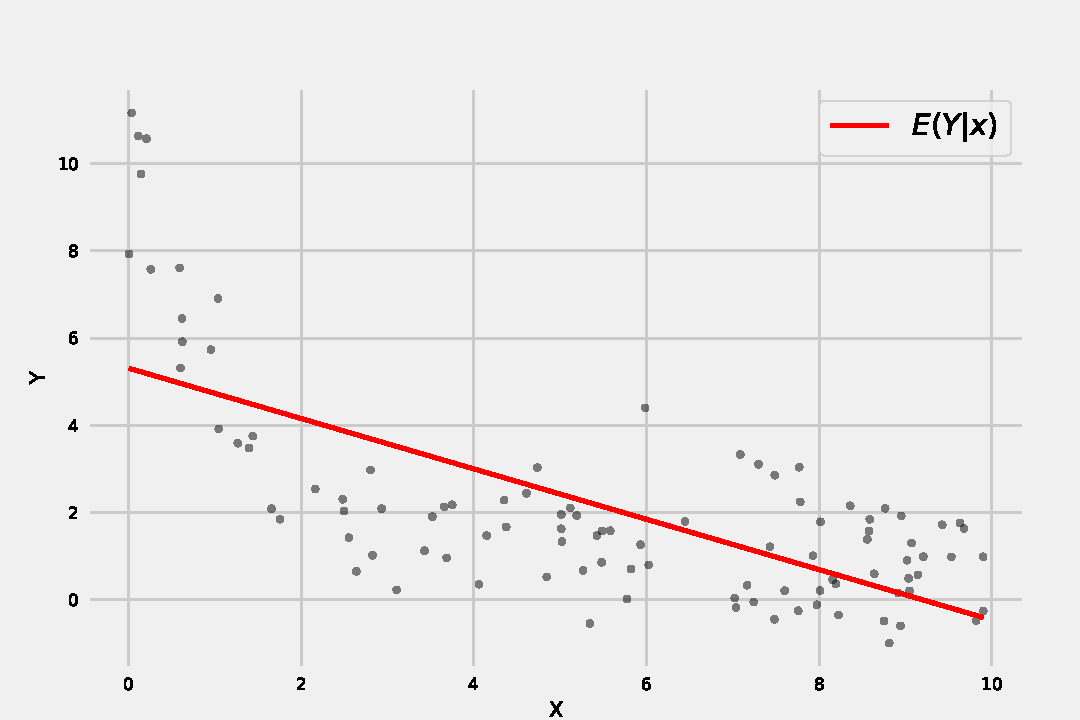
\includegraphics{chapters/chapter7/nonlinear_relationship.pdf}
    \end{figure}
    
    Please sketch what you would expect the residual vs fitted value plot to look like.
    
    \item Suppose that you fit a linear regression model and compute the residuals.
    As the residuals move closer to the line $\mathbb{E}(Y|x)$ will your estimate of $\sigma^{2}$ be smaller or larger? Why?  
    
    \item A linear regression is fit to a dataset where we collected the number of lbs of sugar an undergraduate student consumes during a week in the Fall semester and their H1Ac level.
    We estimate our parameters and find that $\hat{\beta_{0}} = 2$ and $\hat{\beta_{1}} = 10$. It may (or may not) be more reasonable to express the change in H1Ac not in increments of 1lb but instead in increments of 1 ounce.
    Please reexpress the estimated change in H1Ac in ounces of sugar consumed.  
    
    \item Will different parameter estimates lead to different diagnostic plots? Why or why not?
    
    \item The loglikelihood for single covariate regression is 
    \begin{align}
        \ell \ell (\beta_{0}, \beta_{1}, \sigma^{2}) = - \frac{N}{2} \log \left(2 \pi \sigma^{2}\right) - \frac{1}{2 \sigma^{2}} \sum_{i=1}^{n} \left\{   \left \left[y_{i} - (\beta_{0} + \beta_{1}x_{i}) \right]^{2} \right\}
    \end{align}
    We will compute the maximum likelihood estimate for $\beta_{1}$ in a series of steps.
    \begin{enumerate}
        \item Are only variable of interest is $\beta_{1}$. The paramters $\beta_{0}$ and $\sigma^{2}$ can be thought of as constants. Remove any terms in the loglikelihood that are constants. Call this new function $g$
        
        \item Compute the derivative of $g(\beta_{1})$, treating $\beta_{1}$ as a variable.
        
        \item Set $g'(\beta_{1}) = 0$ and solve for $\beta_{1}$ 
        
    \end{enumerate}
    
    \item We saw that we can compute estimates for $\beta_{0}$ and $\beta_{1}$ by minimizing the sums of squares or by maximum likelihood. 
    Please describe how the sums of squares estimates and maximum likelihood estimates are related and why they are related.
    
    \item Why can minimizing the sums of squares function $SS(\beta_{0}, \beta_{1})$ be interpreted as finding the values $(\beta_{0}), \beta_{1}$ that minimize \textbf{the sum} of squared residuals? Why can this minimizatoin be interpreted as minimizing \textbf{the mean} of squared residuals?
    
    \item Suppose we collect the dataset
    \begin{table}[ht!]
        \centering
        \begin{tabular}{c|c}
            x & y \\
            \hline
            -0.72 &  -3.33\\
            -0.78 &  -2.15\\
            -0.69 &  -1.94\\
            -0.12 &  -0.68\\
             0.70 &  0.20\\
            -0.30 &  -0.47\\
            -0.15 &  -2.20\\
            -0.71 &  -1.37\\
            -0.49 &  -1.16\\
             0.92 &  1.77\\
        \end{tabular}
    \end{table}
    \begin{enumerate}
        \item Compute the maximum likelihood estimate for $\beta_{0}$
        \item Compute the maximum likelihood estimate for $\beta_{1}$
        \item Compute the maximum likelihood estimate for $\sigma^{2}$
    \end{enumerate}
    
    \item Suppose we collect the dataset
    \begin{table}[ht!]
        \centering
        \begin{tabular}{c|c}
            x & y \\
            \hline
            -0.49 &  -2.20\\
            -0.55 &  -1.01\\
            -0.46 &  -0.80\\
             0.11 &  0.46\\
             0.93 &  1.34\\
            -0.07 &  0.66\\
             0.08 &  -1.07\\
            -0.48 &  -0.24\\
            -0.26 &  -0.03\\
             1.15 &  2.90\\
        \end{tabular}
    \end{table}
    \begin{enumerate}
        \item Compute the maximum likelihood estimate for $\beta_{0}$
        \item Compute the maximum likelihood estimate for $\beta_{1}$
        \item Compute the maximum likelihood estimate for $\sigma^{2}$
    \end{enumerate}
    
\end{enumerate}





